\chapter{Modelagem matemática }

\section{Descrição do problema}
O problema em análise considera um trem com diferentes tipos de assentos que realizará uma viagem entre uma estação de origem \( E_1 \) e uma estação de destino final \( E_n \) (onde \( n \) representa a última estação da rota). Esse trem terá um itinerário que inclui o nome do trem, a estação de origem, a estação de destino, bem como a data e o horário de partida.

Os assentos disponíveis são classificados conforme suas características — por exemplo, VIP, padrão, entre outros. Para cada tipo de assento, será definida uma lista de preços a ser disponibilizada para venda. Cada preço dessa lista é denominado \textit{classe de controle} (control class). Os bilhetes serão oferecidos ao público antes da partida do trem, sendo o intervalo entre o início das vendas e o momento da partida denominado \textit{horizonte de reserva}. Esse horizonte será segmentado em diversos períodos, que podem adotar diferentes granularidades temporais, como dias, semanas ou meses, inclusive de forma combinada. Os períodos são organizados de forma decrescente, sendo que o valor zero corresponde à data de partida, e o maior valor representa o início da disponibilização dos bilhetes, formando a sequência \( [t, t-1, t-2, ..., 0] \).

Diante dessas condições, o objetivo é controlar a disponibilidade de assentos — tanto os reservados quanto os autorizados para venda — em cada período do horizonte de reserva, visando à maximização do lucro total obtido com a comercialização dos assentos reservados.

Para alcançar esse objetivo, o modelo deve considerar restrições que assegurem: a capacidade física do trem, a integridade das variáveis inteiras, a relação entre os assentos reservados e a demanda, bem como a coerência entre os assentos reservados e os efetivamente disponibilizados para venda.

Essas restrições compõem o \textit{modelo básico}. No entanto, esta pesquisa propõe a inserção de dois conjuntos adicionais de restrições, que, segundo os autores, refletem práticas amplamente utilizadas em ambientes reais. Esses conjuntos são: as restrições do tipo \textbf{ \textit{Fulfillments over Periods}}, relacionadas a condições temporais; e as restrições do tipo \textbf{\textit{Skip Lagging}}, associadas ao padrão de paradas do trem. Onde, o primeiro conjunto garante que: i) Os preços das classes de controle ofertadas devem aumentar progressivamente à medida que se aproxima a data de partida do trem; ii) Uma determinada classe de controle para um trecho específico só poderá ser reservada se já tiver sido reservada em um período anterior dentro do horizonte de reserva.

Já o segundo conjunto assegura que: i) Os passageiros não possam adquirir bilhetes para estações posteriores com a intenção de desembarcar antes do destino indicado no bilhete. Ou seja, para uma origem dada, os preços das passagens para destinos mais distantes devem ser proporcionais à distância percorrida; ii) Para um par origem-destino, a soma dos preços dos trechos intermediários contínuos não deve ser inferior ao valor de uma passagem direta.

Por fim, é importante destacar um conceito essencial: o tipo de demanda considerado. Neste trabalho, serão utilizadas duas abordagens: a \textbf{Demanda independente}: caracterizada por decisões de compra que não consideram a oferta disponível no momento da compra; e a \textbf{Demanda comportamental}: baseada em listas de preferência, nas quais os passageiros escolhem entre diferentes preços conforme sua disponibilidade e preferências no momento da compra.


\section{Formulação matemática}

% Como mencionado anteriormente, esta pesquisa propõe três modelos matemáticos de programação inteira mista. O primeiro utiliza uma demanda do tipo independente; o segundo emprega um modelo de demanda comportamental ajustado por proporções, onde essas proporções são calculadas com base na demanda independente; e o terceiro adota um modelo de demanda comportamental ajustado por hierarquia, em que essa hierarquia está associada à quantidade de assentos reservados para cada classe de controle.

Para facilitar a compreensão da proposta, apresenta-se a seguir uma versão simplificada do problema, conforme ilustrado na Figura \ref{fig: fig1}, na qual são considerados os seguintes elementos:

\begin{itemize}
	\setlength{\itemsep}{-0.5em} % Ajusta el interlineado entre ítems
	\item 4 estações pelas quais o trem deve passar em um único sentido, ou seja, o trem não tem retorno.
	\item O trem tem uma capacidade física máxima de assentos;
	\item Há apenas um tipo de classe de controle;
	\item Existe apenas um período no horizonte de reserva;
	\item Considera-se, neste caso, apenas a variável de decisão associada à quantidade de assentos reservados em um trecho com origem e destino específicos;
	\item Todos os assentos reservados serão vendidos;
	\item É considerada um tipo de demanda independente;
	\item É considerada somente a restrição de capacidade física do trem.
\end{itemize}

\begin{figure}[H]
	\begin{center}
		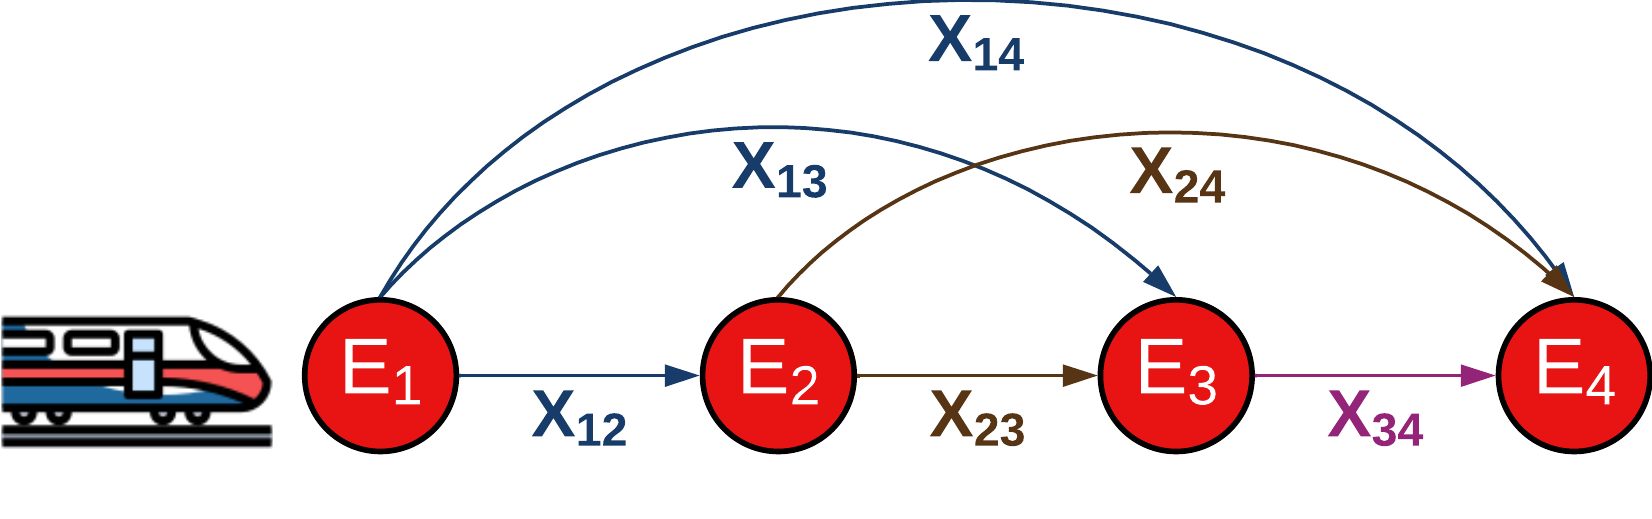
\includegraphics[scale=0.18]{img/repre_ini1.png}
		\caption{Versão gráfica simples do Problema de Transporte Ferroviário de Passageiros}
		% Fonte:~\cite{khaksar2013genetic}}
		\label{fig: fig1}
	\end{center}
\end{figure}
\vspace{-1cm}

Com base no exposto, é possível definir os seguintes parâmetros e variáveis de decisão:

\begin{description}[style=unboxed, leftmargin=2.5cm, labelindent=1.5cm]
	\setlength{\itemsep}{-2.2em} % Ajusta el interlineado entre ítems
	\setlength{\parskip}{0em} % Espaciado entre párrafos
	\item[$x_{ij}$]: Quantidade de assentos que serão reservados no trecho com origem em $i$ e destino em $j$, onde $j>i$ (variável de decisão); \\
	\item[$A_i$]: Quantidade de assentos vagos na estação $i$; \\
	\item[$P_{ij}$]: Preço da passagem no trecho com origem em $i$ e destino em $j$; \\
	\item[$Q$]: Capacidade física do trem.
\end{description}



Assim, a função objetivo será maximizar o lucro para cada possível reserva em cada trecho $i,j$, matematicamente seria:

$FO: max \quad x_{12}P_{12} + x_{13}P_{13} + x_{14}P_{14} + x_{23}P_{23} + x_{24}P_{24} + x_{34}P_{34}$

s.a.

Estação 1: $x_{12} + x_{13} + x_{14} \leq A_1 \quad onde \quad A_1 = Q $ \\
\indent Estação 2: $x_{23} + x_{24}  \leq  A_2 \quad onde \quad A_2 = A_1 - (x_{12} + x_{13} + x_{14}) + x_{12} $ \\
\indent Estação 3: $x_{34} \leq A_3 \quad onde \quad A_3 = A_2 - (x_{23} + x_{24}) + x_{13} + x_{23} $

Observe que as restrições de capacidade são aplicadas apenas às três primeiras estações — $E_1, E_2$ e $E_3$ —, já que são as únicas que possuem pelo menos um destino associado. A estação $E_4$ é excluída, pois não possui nenhum destino.

Cada uma das restrições leva em consideração o fluxo de pessoas que sairão e entrarão no trem. Levando isso em conta, é necessário calcular a quantidade de assentos vagos do trem para cada estação. Considere uma solução viável para o modelo, conforme mostrado na Figura \ref{fig: fig2}, com uma capacidade total de 100 assentos para um trem.

\begin{figure}[H]
	\begin{center}
		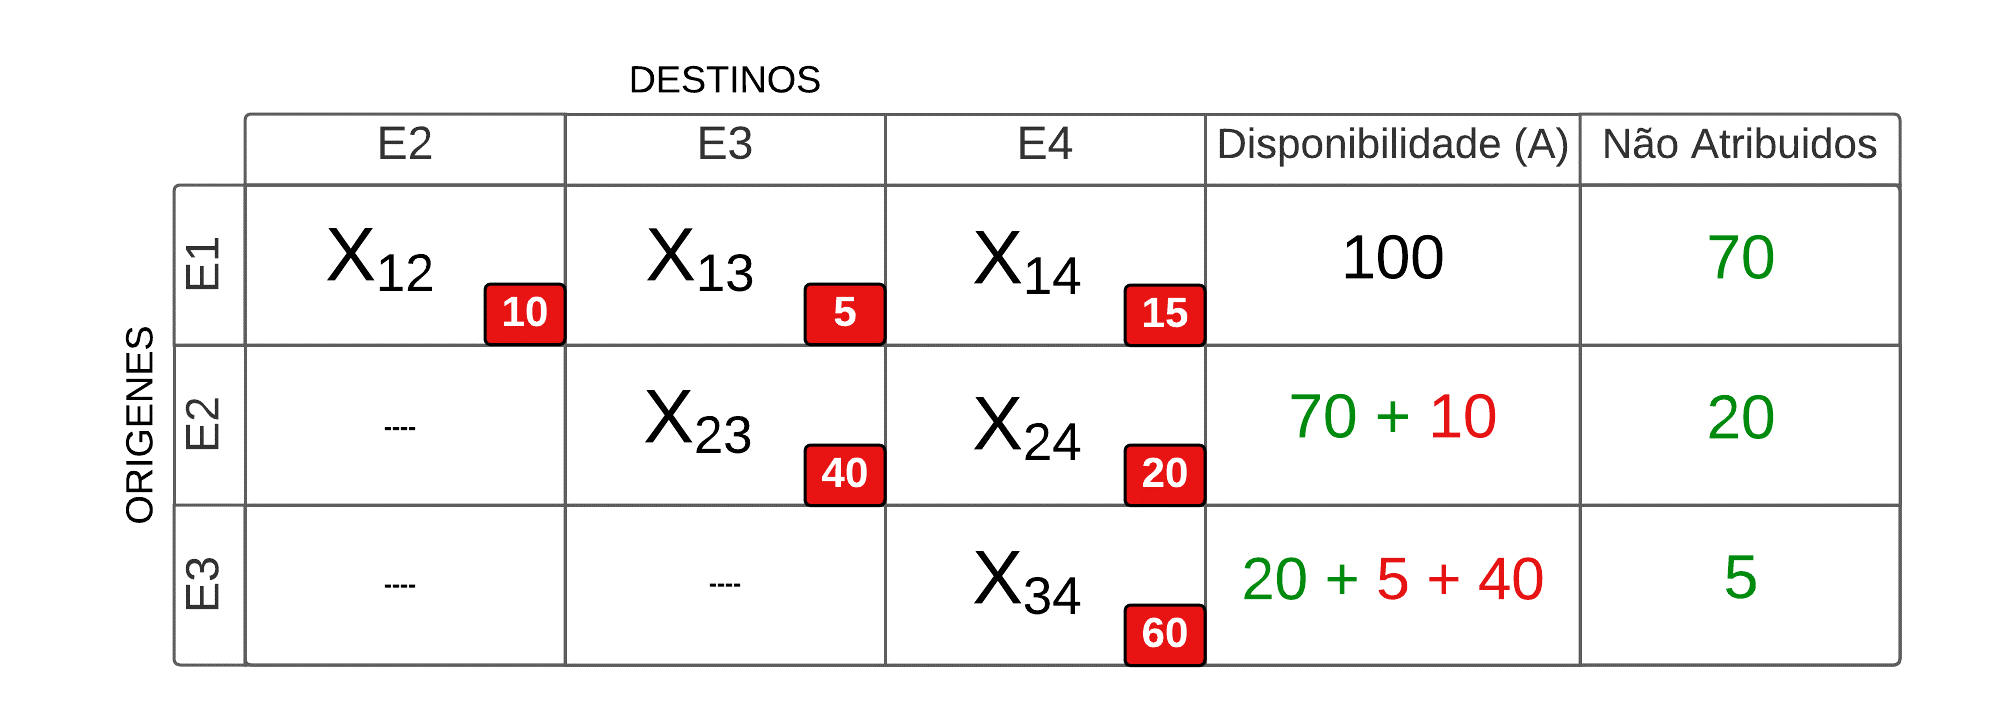
\includegraphics[scale=0.4]{img/fig2.png}
		\caption{Solução factível para o problema simplificado}
		% Fonte:~\cite{khaksar2013genetic}}
		\label{fig: fig2}
	\end{center}
\end{figure}
\vspace{-1cm}

Note que, para a restrição da estação 1, o trem está com todos os assentos vazios, ou seja, \(A_1=100\), e que a soma das variáveis seria \(x_{12} + x_{13} + x_{14} = 10 + 5 + 15 = 30\). Portanto, a restrição é satisfeita com \(30 \leq 100\), ou seja, foram reservados 30 assentos dos 100 que o trem possui. Nesse sentido, no momento da partida do trem da estação 1, haveria 70 assentos vazios ou disponíveis para reservar em estações posteriores.

Agora, para a estação 2, teríamos \(A_2 = 100 - 30 + 10 = 70 + 10 = 80\). Já era conhecido que havia 70 assentos disponíveis vindos da estação 1, mas também é preciso levar em conta que os assentos com destino à estação 2 também ficarão disponíveis da estação 2 em diante, para este caso \(x_{12} = 10\). Portanto, para a estação 2, teríamos 80 assentos vazios para reservar, é assim que a restrição é cumprida com \(60 \leq 80\). Analogamente, o mesmo raciocínio seria aplicado para a estação 3, ou seja, teríamos a soma de todos os assentos que chegaram à estação 3, \(x_{13} = 5\) e \(x_{23} = 40\), assim teríamos \(A_3 = 80 - 60 + 5 + 40 = 20 + 5 + 40 = 65\), e no final, a restrição é satisfeita com \(60 \leq 65\).


% Cada relação possível entre uma estação e outra será denominada origem-destino ou trecho. Será dito que uma origem-destino é adjacente se, e somente se, não houver estações intermediárias entre elas; caso contrário, serão não adjacentes. Por exemplo, na Figura \ref{fig: fig1}, os trechos adjacentes seriam: $(E_1-E_2)$, $(E_2-E_3)$, $(E_3-E_4)$, e os trechos não adjacentes seriam: $(E_1-E_3)$, $(E_1-E_4)$ e $(E_2-E_4)$. Além disso, observe que os trechos não adjacentes podem conter outros trechos, tanto adjacentes quanto não adjacentes. Por exemplo, o trecho $(E_1-E_4)$ da Figura \ref{fig: fig1} contém os trechos adjacentes $(E_1-E_2)$, $(E_2-E_3)$, e contém os trechos não adjacentes $(E_1-E_3)$ e $(E_2-E_4)$. Vejamos o modelo completo:


Nas seções seguintes, para cada abordagem, serão apresentados os modelos completos, iniciando por um modelo base. Em seguida, a esse modelo base serão adicionados, de forma separada, tanto os conjuntos de restrições do tipo Skip Lagging quanto os conjuntos de restrições do tipo Fulfillment. Por fim, também será apresentado o modelo completo, no qual todos os conjuntos de restrições são incorporados simultaneamente.

\section{Primeira abordagem: modelo baseado em demanda independente}\label{sec:modelo1}

Nos modelos desta seção, considera-se uma demanda independente, ou seja, assume-se que cada cliente realiza sua decisão de compra de forma isolada em relação à oferta disponível no momento da aquisição. Em termos práticos, isso implica que, se um passageiro estiver disposto a pagar, por exemplo, R\$10 por um determinado assento, ele efetuará a compra apenas se encontrar esse valor específico, mesmo que existam tarifas mais baixas disponíveis. Caso não encontre o preço correspondente à sua disposição de pagamento, optará por não realizar a compra.

\subsection{Modelo básico independente}
O modelo base é composto pelas restrições fundamentais que estruturam o problema em estudo. Essas restrições definem os limites operacionais e lógicos essenciais para garantir a viabilidade da solução, refletindo as condições básicas do sistema ferroviário de transporte de passageiros, como a capacidade física do trem, a integridade das variáveis inteiras, a relação entre os assentos reservados e a demanda, bem como a coerência entre os assentos reservados e os efetivamente disponibilizados para venda.

% Antes de apresentar os modelos completos e generalizados, são descritos a seguir todos os conjuntos, parâmetros e variáveis de decisão necessários para sua compreensão adequada. Essa etapa é essencial para garantir clareza na formulação matemática e no entendimento das relações que compõem a estrutura do modelo.

Então, para esta proposta considere os seguintes conjuntos:

\begin{description}[style=unboxed, leftmargin=2.5cm, labelindent=1.5cm]
	\setlength{\itemsep}{-2.2em} % Ajusta el interlineado entre ítems
	\setlength{\parskip}{0em} % Espaciado entre párrafos
	\item[$O:$] Conjunto de estações de origem. \\
	\item[$D:$] Conjunto de estações de destino. \\
	\item[$OD:$] Conjunto de trechos com itinerário. \\
	      % \item[$NAD:$] Conjunto de trechos que NÃO são adjacentes e que tem itinerário.\\
	      % \item[$BRI_{(o,d)}:$] Conjunto de trechos contidos dentro de cada trecho $(o,d)$ não adjacente.\\
	      % \item[$CR_{(o,d)}:$] É um conjunto que contém outros subconjuntos, onde cada subconjunto é uma rota possível para ir desde a origem $o$ até o destino $d$, sendo $(o,d)$ não adjacente. \\
	      % \item[$S:$] Representa cada subconjunto dentro de $CR_{(o,d)}$. \\
	\item[$V:$] Conjunto de tipos de assento do trem. \\
	\item[$T:$] Conjunto de períodos. \\
	\item[$K_v:$] É o conjunto de classes de controle para cada tipo de assento $v$. Onde os índices de cada $K_v$ estão em ordem decrescente, enquanto seus valores são crescentes.
\end{description}

Considere os seguintes parâmetros:
\begin{description}[style=unboxed, leftmargin=2.5cm, labelindent=1.5cm]
	\setlength{\itemsep}{-2.2em} % Ajusta el interlineado entre ítems
	\setlength{\parskip}{0em} % Espaciado entre párrafos
	% \item[$n:$] Quantidade de estações.\\
	\item[$Q_v:$] Capacidade física do trem para cada tipo de assento $v$, onde $v \in V$. \\
	\item[$P_{ijvk}:$] Preços  das passagens no trecho $(i,j)$, tipo de assento $v$ e classe de controle $k$, onde $(i,j) \in OD,v \in V, k \in K_v$.  \\
	\item[$d_{ijvkt}:$] Demanda independente no trecho $(i,j)$, tipo de assento $v$ e classe de controle $k$, onde $(i,j) \in OD,v \in V, k \in K_v, t \in T$.
	      % \item[$d'_{ijvkt}:$] Demanda comportamental no trecho $(i,j)$, tipo de assento $v$ e classe de controle $k$, onde $(i,j) \in OD,v \in V, k \in K_v, t \in T$.
\end{description}

Considere as seguintes variáveis de decisão:
\begin{description}[style=unboxed, leftmargin=2.5cm, labelindent=1.5cm]
	\setlength{\itemsep}{-2.2em} % Ajusta el interlineado entre ítems
	\setlength{\parskip}{0em} % Espaciado entre párrafos
	\item[$X_{ijvkt}:$] Quantidade de passagens reservadas no trecho $(i,j)$, tipo de assento $v$ e com classe de controle $k$ no período $t$, onde $(i,j) \in OD, v \in V, k \in K_v, t \in T$.  \\
	\item[$Y_{ijvk}:$] Quantidade de passagens autorizadas no trecho $(i,j)$, tipo de assento $v$ e com classe de controle $k$, onde $(i,j) \in OD, v \in V, k \in K_v$.
	      % \item[$\gamma_{ijvkt}:$] É uma variável binaria que toma o valor de 1 quando $Y_{ijvkt} \neq 0$ e toma  valor de 0 caso contrario, onde $(i,j) \in OD, v \in V, k \in K_v, t \in T$. \\
	      % \item[$\beta_{ijvkt}:$] É uma variável binaria que toma o valor de 1 quando a classe $k$ é a classe mais barata que foi autorizada para venda, no trecho $(i,j)$, tipo de assento $v$ e período $t$; e toma  valor de 0 caso contrario, onde $(i,j) \in OD, v \in V, k \in K_v, t \in T$.  \\
	      % \item[$\alpha_{ijvkt}:$] É uma variável binaria que toma o valor de 1 quando $X_{ijvkt} \neq 0$ e toma  valor de 0 caso contrario, onde $(i,j) \in OD, v \in V, k \in K_v, t \in T$.
\end{description}

Considere a seguinte variável auxiliar:
\begin{description}[style=unboxed, leftmargin=2.5cm, labelindent=1.5cm]
	\setlength{\itemsep}{-2.2em} % Ajusta el interlineado entre ítems
	\setlength{\parskip}{0em} % Espaciado entre párrafos
	\item[$A_{iv}:$] Armazena a quantidade de assentos vazios disponíveis para venda em cada estação de origem $i$ e cada tipo de assento $v$ durante todo o horizonte de reserva, onde $i \in O, v \in V$. Cabe esclarecer que esta não é uma variável de decisão, pois esta variável apenas armazena um cálculo com base na capacidade física do trem e nas variáveis de decisão de passagens reservadas.
\end{description}

\noindent \textbf{Modelo}
\begin{equation}
	Max \quad Z = \sum_{(i,j)\in OD} \sum_{v\in V} \sum_{k\in K_v} \sum_{t\in T} P_{ijvk} X_{ijvkt}           \label{eq: m1_fo}
\end{equation}
Em primeiro lugar, define-se a função objetivo conforme apresentada na equação \eqref{eq: m1_fo}. Observa-se que seu propósito é maximizar a receita total, considerando as quantidades de assentos reservados para cada combinação de trechos, tipo de assento, classes de controle e periodos, ponderadas pelos respectivos preços associados.
\begin{equation}
	A_{iv} = A_{i-1,v} - \sum_{(i,j) \in OD/j \geq i} \sum_{k\in K_v}\sum_{t\in T}X_{i-1,j,v,k,t} + \sum_{(i,j) \in OD/j<i} \sum_{k\in K_v}\sum_{t\in T}X_{jivkt}, \quad \forall i \in O, v \in V  \label{eq: m1_disponi}
\end{equation}
A restrição \eqref{eq: m1_disponi} tem como finalidade calcular, de forma sistemática, a quantidade de assentos disponíveis em cada estação de origem em todo o horizonte de reserva. Essa formulação representa uma generalização do procedimento apresentado no exemplo simplificado utilizado anteriormente para o cálculo de $A_{i}$, expandindo-o para capturar a dinâmica completa do sistema ao longo do tempo, entre múltiplas classes de controle e considerando cada tipo de assento de forma específica.
\begin{equation}
	Y_{ijvk} \geq  \sum_{t \in T} X_{ijvkt},  \quad k = max\{K_v\}, \forall(i,j) \in OD ,v \in V    \label{eq: m1_autho_mayor_assig_1er_class}
\end{equation}
\begin{equation}
	Y_{ijvk} \geq  \sum_{t \in T} X_{ijvkt} + Y_{i,j,v,k + 1} , \quad \forall(i,j) \in OD, v \in V, k \in K_v / k < \lVert K_v \rVert  \label{eq: m1_autho_mayor_assig_mas_autho}
\end{equation}
A variável de decisão $Y_{ijvk}$ adota uma estrutura do tipo nesting, onde cada classe tarifária mais cara (classe “pai”) engloba todas as classes mais baratas (classes “filhas”). Nesse encadeamento, todas as classes possuem um pai e um filho, com exceção da classe mais cara — que não possui pai — e da classe mais barata — que não possui filho. Dessa forma, o valor mínimo da variável $Y_{ijvk}$ para uma determinada classe deve ser igual ou superior à soma das reservas dessa própria classe e das autorizações concedidas à sua classe filha (como visto na Figura \ref{fig: nesting} para as classes $1, 2, 3$). A restrição \eqref{eq: m1_autho_mayor_assig_1er_class} formaliza esse comportamento especificamente para a classe mais barata, enquanto a restrição \eqref{eq: m1_autho_mayor_assig_mas_autho} garante essa hierarquia para as demais classes de controle.
\begin{figure}[H]
	\begin{center}
		\begin{tikzpicture}[
				boxY/.style={rectangle, minimum width=2.2cm, minimum height=0.8cm, rounded corners=2pt, fill=red!70, text=white, font=\bfseries, align=center},
				boxX/.style={rectangle, minimum width=1.5cm, minimum height=0.8cm, rounded corners=2pt, fill=teal!80, text=white, font=\bfseries, align=center},
				arrow/.style={-Latex, thick, blue!70},
				every node/.style={inner sep=3pt}
			]

			% Nodos
			\node[boxY] (y1) at (0,0) {Y$_{12P\textcolor{black}{1}}$};
			\node[boxX] (x1) at (2.7,0) {$\sum_{t \in T} X_{12P\textcolor{black}{1}t}$};

			\node[boxY] (y2) at (2.7,-1.1) {Y$_{12P\textcolor{black}{2}}$};
			\node[boxX] (x2) at (5.4,-1.1) {$\sum_{t \in T} X_{12P\textcolor{black}{2}t}$};

			\node[boxY] (y3) at (5.4,-2.2) {Y$_{12P\textcolor{black}{3}}$};
			\node[boxX] (x3) at (8.1,-2.2) {$\sum_{t \in T} X_{12P\textcolor{black}{3}t}$};

			% Flechas (curvas según la imagen original)
			\draw[arrow] (y1.east) -- (x1.west);
			\draw[arrow] (y1.east) to[out=-20,in=180] (y2.west);
			\draw[arrow] (y2.east) -- (x2.west);
			\draw[arrow] (y2.east) to[out=-20,in=180] (y3.west);
			\draw[arrow] (y3.east) -- (x3.west);

			% Texto explicativo
			% \node[align=left] at (-0.3,-5.3) {
			% 	\small Trecho: 12\\
			% 	\small Tipo assento: P
			% };

		\end{tikzpicture}
	\end{center}
	\caption{Exemplo de nesting para o trecho $E_1 - E_2$ e tipo de assento $P$}
	\label{fig: nesting}
\end{figure}

\vspace{-1cm}

\begin{equation}
	\sum_{(i,j) \in OD} Y_{ijvk} \leq A_{iv}, \quad  k = min\{K_v\}, \forall i \in O / (i,j) \in OD,   \forall v \in V      \label{eq: m1_cap_autho_1er_class}
\end{equation}
Considerando que a variável $Y_{ijvk}$ é do tipo nesting e levando em conta as duas restrições \eqref{eq: m1_autho_mayor_assig_1er_class} e \eqref{eq: m1_autho_mayor_assig_mas_autho}, fica evidente que a classe mais cara engloba as quantidades das demais classes; portanto, deve-se assegurar que ela não exceda o número de assentos vazios. Essa condição é garantida pela restrição \eqref{eq: m1_cap_autho_1er_class}.
\begin{equation}
	X_{ijvkt} \leq d_{ijvkt},  \quad \forall (i,j) \in OD / i < j  ,v \in V, k \in K_v, t\in T  \label{eq: m1_assig_menor_dem}
\end{equation}
A restrição \eqref{eq: m1_assig_menor_dem} assegura que, para cada trecho, classe, tipo de assento e período do horizonte de reserva, a quantidade de passagens reservadas não exceda a demanda correspondente.
\allowdisplaybreaks
\begin{gather}
	A_{0,v} = Q_v \quad \forall v \in V \label{eq: m1_ini_disponi} \\
	X_{0,j,v,k,t} = 0 \quad \forall j \in D,\, v \in V,\, k \in K_v,\, t \in T \label{eq: m1_ini_assig} \\
	X_{ijvkt} \in \mathbb{Z}^+ \quad \forall(i,j) \in OD,\, v \in V,\, k \in K_v,\, t \in T \label{eq: m1_dom_assig} \\
	Y_{ijvk} \in \mathbb{Z}^+ \quad \forall(i,j) \in OD,\, v \in V,\, k \in K_v \label{eq: m1_dom_autho} \\
	A_{iv} \in \mathbb{Z}^+ \quad \forall i \in O,\, v \in V \label{eq: m1_dom_disponi}
\end{gather}

As restrições \eqref{eq: m1_ini_disponi} e \eqref{eq: m1_ini_assig} são usadas para inicializar a restrição \eqref{eq: m1_disponi} quando \(i = 1\). E as restrições de \eqref{eq: m1_dom_assig} a \eqref{eq: m1_dom_disponi} representam o domínio das variáveis.

Assim, o \textbf{modelo básico} seria o seguinte:
\allowdisplaybreaks
\begin{align}
	& Max \quad Z = \sum_{(i,j)\in OD} \sum_{v\in V} \sum_{k\in K_v} \sum_{t\in T} P_{ijvk} X_{ijvkt}     \tag{\ref{eq: m1_fo}}   \\
	& \text{s.a.}  \notag \\
	& A_{iv} = A_{i-1,v} - \sum_{(i,j) \in OD/j \geq i} \sum_{k\in K_v}\sum_{t\in T}X_{i-1,j,v,k,t} + \sum_{(i,j) \in OD/j<i} \sum_{k\in K_v}\sum_{t\in T}X_{jivkt}, \quad \forall i \in O, v \in V   \tag{\ref{eq: m1_disponi}} \\
	& Y_{ijvk} \geq  \sum_{t \in T} X_{ijvkt},  \quad k = max\{K_v\}, \forall(i,j) \in OD ,v \in V     \tag{\ref{eq: m1_autho_mayor_assig_1er_class}} \\
	& Y_{ijvk} \geq  \sum_{t \in T} X_{ijvkt} + Y_{i,j,v,k + 1} , \quad \forall(i,j) \in OD, v \in V, k \in K_v / k < \lVert K_v \rVert   \tag{\ref{eq: m1_autho_mayor_assig_mas_autho}} \\
	& \sum_{(i,j) \in OD} Y_{ijvk} \leq A_{iv}, \quad  k = min\{K_v\}, \forall i \in O / (i,j) \in OD,   \forall v \in V       \tag{\ref{eq: m1_cap_autho_1er_class}} \\
	& X_{ijvkt} \leq d_{ijvkt},  \quad \forall (i,j) \in OD / i < j  ,v \in V, k \in K_v, t\in T   \tag{\ref{eq: m1_assig_menor_dem}} \\
	& A_{0,v} = Q_v \quad \forall v \in V  \tag{\ref{eq: m1_ini_disponi}} \\ 
	& X_{0,j,v,k,t} = 0 \quad \forall j \in D,\, v \in V,\, k \in K_v,\, t \in T  \tag{\ref{eq: m1_ini_assig}} \\ 
	& X_{ijvkt} \in \mathbb{Z}^+ \quad \forall(i,j) \in OD,\, v \in V,\, k \in K_v,\, t \in T  \tag{\ref{eq: m1_dom_assig}} \\ 
	& Y_{ijvk} \in \mathbb{Z}^+ \quad \forall(i,j) \in OD,\, v \in V,\, k \in K_v  \tag{\ref{eq: m1_dom_autho}} \\ 
	& A_{iv} \in \mathbb{Z}^+ \quad \forall i \in O,\, v \in V  \tag{\ref{eq: m1_dom_disponi}} 
\end{align}

\subsection{Modelo fulfillments over periods independente}
Lembrando que as restrições do tipo fulfillment over periods referem-se ao atendimento de determinados níveis de serviço, demanda ou capacidade ao longo do horizonte de reservas, este modelo adiciona, ao modelo básico, um conjunto de restrições que definem quando assentos em determinadas classes devem ser reservados ou não. Além disso, 
deve-se garantir algumas regras para os precos das classes em função do tempo. Para este fim, devem ser adicionadas as seguintes variáveis de decisão:

\begin{description}[style=unboxed, leftmargin=2.5cm, labelindent=1.5cm]
	\setlength{\itemsep}{-2.2em} % Ajusta el interlineado entre ítems
	\setlength{\parskip}{0em} % Espaciado entre párrafos
	\item[$\beta_{ijvkt}:$] É uma variável binaria que toma o valor de 1 quando a classe $k$ é a classe mais barata que foi autorizada para venda, no trecho $(i,j)$, tipo de assento $v$ e período $t$; e toma  valor de 0 caso contrario, onde $(i,j) \in OD, v \in V, k \in K_v, t \in T$.  \\
	\item[$\alpha_{ijvkt}:$] É uma variável binaria que toma o valor de 1 quando $X_{ijvkt} \neq 0$ e toma  valor de 0 caso contrario, onde $(i,j) \in OD, v \in V, k \in K_v, t \in T$.
\end{description}
\textbf{Restrições:}
\begin{equation}
	\alpha_{ijvkt} \leq X_{ijvkt} \leq \alpha_{ijvkt}d_{ijvkt}, \quad   \forall(i,j) \in OD, v \in V, k \in K_v, t \in T   \label{eq: m1_binaria_alpha}
\end{equation}
A restrição  \eqref{eq: m1_binaria_alpha} é utilizada para determinar quando a variável de decisão $X$ assume valores diferentes de zero e quando não. Assim, $\alpha$ toma o valor de 1 no primeiro caso e 0 no segundo.
\begin{equation}
	\beta_{ijvkt} = \alpha_{ijvkt} - \alpha_{i,j,v,k+1,t}, \quad \forall (i,j) \in OD, v \in V, k \in K /k < max\{K_v\}, t\in T    \label{eq: m1_binaria_Beta}
\end{equation}
\begin{equation}
	\beta_{ijvkt} = \alpha_{ijvkt}, \quad   \forall(i,j) \in OD, v \in V, k = max\{K_v\}, t \in T    \label{eq: m1_binaria_Beta_last}
\end{equation}
As restrições \eqref{eq: m1_binaria_Beta} e \eqref{eq: m1_binaria_Beta_last} têm como objetivo identificar a classe de assento mais barata reservada em um determinado trecho, tipo de assento e período. A restrição \eqref{eq: m1_binaria_Beta} é utilizada exclusivamente para as classes mais baratas, enquanto a restrição \eqref{eq: m1_binaria_Beta_last} se aplica às demais classes de assento. Assim, a variável $\beta$ assume o valor de 1 quando a classe $k$ é a mais barata reservada e 0 caso contrário (veja a Figura \ref{fig: betha}).
\begin{figure}[H]
	\begin{center}
		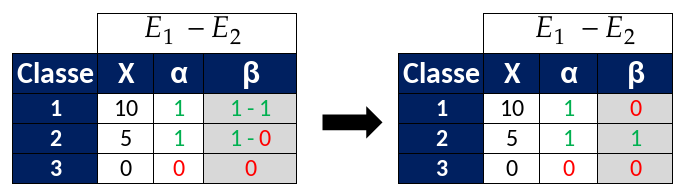
\includegraphics[scale=0.45]{img/betha.png}
		\caption{Exemplo cálculo da variável $\beta$ para o trecho $E_1 - E_2$, um período e um tipo de assento}
		\label{fig: betha}
	\end{center}
\end{figure}

\vspace{-1cm}

\begin{equation}
	\alpha_{ijvkt} \leq \alpha_{i,j,v,k,t+1}, \quad   \forall(i,j) \in OD, v \in V, k \in K_v, t \in T/ t \neq max\{T\}     \label{eq: m1_assig_last_periodo}
\end{equation}
Uma condição importante estabelece que uma classe pode ser reservada desde que essa mesma classe já tenha sido reservada em períodos anteriores. Para isso, definem-se a restrição \eqref{eq: m1_assig_last_periodo}. Cabe lembrar que o tempo $t$ representa os $t$ períodos antes da saída do trem, sendo que a partida do trem ocorre em $t = 0$.
\begin{equation}
	\sum_{k \in K_v}\beta_{ijvkt}P_{ijvk} \geq \sum_{k \in K_v}\beta_{i,j,v,k,t+1}P_{ijvk},  \quad   \forall(i,j) \in OD, v \in V, t \in T/ t \neq max\{T\}   \label{eq: m1_fulfill_periodo}
\end{equation}
Outra condição especial deste problema está relacionada à disponibilização dos preços dos bilhetes ao longo do tempo. Esses preços devem seguir uma lógica contínua, sem oscilações. Em outras palavras, os preços dos bilhetes devem sempre aumentar conforme a data de partida do trem se aproxima. A restrição \eqref{eq: m1_fulfill_periodo} é responsável por garantir que essa condição seja atendida.

Assim, o \textbf{modelo fulfillments over periods} seria o seguinte:
\allowdisplaybreaks
\begin{align}
	& Max \quad Z = \sum_{(i,j)\in OD} \sum_{v\in V} \sum_{k\in K_v} \sum_{t\in T} P_{ijvk} X_{ijvkt}     \tag{\ref{eq: m1_fo}}   \\
	& \text{s.a.}  \notag \\
	& A_{iv} = A_{i-1,v} - \sum_{(i,j) \in OD/j \geq i} \sum_{k\in K_v}\sum_{t\in T}X_{i-1,j,v,k,t} + \sum_{(i,j) \in OD/j<i} \sum_{k\in K_v}\sum_{t\in T}X_{jivkt}, \quad \forall i \in O, v \in V   \tag{\ref{eq: m1_disponi}} \\
	& Y_{ijvk} \geq  \sum_{t \in T} X_{ijvkt},  \quad k = max\{K_v\}, \forall(i,j) \in OD ,v \in V     \tag{\ref{eq: m1_autho_mayor_assig_1er_class}} \\
	& Y_{ijvk} \geq  \sum_{t \in T} X_{ijvkt} + Y_{i,j,v,k + 1} , \quad \forall(i,j) \in OD, v \in V, k \in K_v / k < \lVert K_v \rVert   \tag{\ref{eq: m1_autho_mayor_assig_mas_autho}} \\
	& \sum_{(i,j) \in OD} Y_{ijvk} \leq A_{iv}, \quad  k = min\{K_v\}, \forall i \in O / (i,j) \in OD,   \forall v \in V       \tag{\ref{eq: m1_cap_autho_1er_class}} \\
	& X_{ijvkt} \leq d_{ijvkt},  \quad \forall (i,j) \in OD / i < j  ,v \in V, k \in K_v, t\in T   \tag{\ref{eq: m1_assig_menor_dem}} \\
	& A_{0,v} = Q_v \quad \forall v \in V  \tag{\ref{eq: m1_ini_disponi}} \\ 
	& X_{0,j,v,k,t} = 0 \quad \forall j \in D,\, v \in V,\, k \in K_v,\, t \in T  \tag{\ref{eq: m1_ini_assig}} \\ 
	& X_{ijvkt} \in \mathbb{Z}^+ \quad \forall(i,j) \in OD,\, v \in V,\, k \in K_v,\, t \in T  \tag{\ref{eq: m1_dom_assig}} \\ 
	& Y_{ijvk} \in \mathbb{Z}^+ \quad \forall(i,j) \in OD,\, v \in V,\, k \in K_v  \tag{\ref{eq: m1_dom_autho}} \\ 
	& A_{iv} \in \mathbb{Z}^+ \quad \forall i \in O,\, v \in V  \tag{\ref{eq: m1_dom_disponi}} \\
	& \textit{\underline{Restrições fulfillments over periods}}         \notag   \\
	& \alpha_{ijvkt} \leq X_{ijvkt} \leq \alpha_{ijvkt}d_{ijvkt}, \quad   \forall(i,j) \in OD, v \in V, k \in K_v, t \in T   \tag{\ref{eq: m1_binaria_alpha}} \\
	& \beta_{ijvkt} = \alpha_{ijvkt} - \alpha_{i,j,v,k+1,t}, \quad \forall (i,j) \in OD, v \in V, k \in K /k < max\{K_v\}, t\in T    \tag{\ref{eq: m1_binaria_Beta}}   \\
	& \beta_{ijvkt} = \alpha_{ijvkt}, \quad   \forall(i,j) \in OD, v \in V, k = max\{K_v\}, t \in T    \tag{\ref{eq: m1_binaria_Beta_last}}   \\
	& \alpha_{ijvkt} \leq \alpha_{i,j,v,k,t+1}, \quad   \forall(i,j) \in OD, v \in V, k \in K_v, t \in T/ t \neq max\{T\}     \tag{\ref{eq: m1_assig_last_periodo}}   \\
	& \sum_{k \in K_v}\beta_{ijvkt}P_{ijvk} \geq \sum_{k \in K_v}\beta_{i,j,v,k,t+1}P_{ijvk},  \quad   \forall(i,j) \in OD, v \in V, t \in T/ t \neq max\{T\}   \tag{\ref{eq: m1_fulfill_periodo}}
\end{align}


\subsection{Modelo skip lagging independente}
A seguir, apresenta-se um modelo que incorpora restrições de skip lagging. O skip lagging envolve a possibilidade de reservar um assento para um destino intermediário, mas com a intenção de não completar a viagem até o destino final. Este modelo propõe restrições que regulam a viabilidade e as condições em que o skip lagging pode ser aplicado, considerando a gestão de capacidade, as políticas de precificação e os níveis de serviço a serem atendidos ao longo do horizonte de reservas. para esse fim, devem ser adicionadas as seguintes:

Variáveis de decisão (mesmas usadas no modelo de fulfillments over periods):
\begin{description}[style=unboxed, leftmargin=2.5cm, labelindent=1.5cm]
	\setlength{\itemsep}{-2.2em} % Ajusta el interlineado entre ítems
	\setlength{\parskip}{0em} % Espaciado entre párrafos
	\item[$\beta_{ijvkt}:$] É uma variável binaria que toma o valor de 1 quando a classe $k$ é a classe mais barata que foi autorizada para venda, no trecho $(i,j)$, tipo de assento $v$ e período $t$; e toma  valor de 0 caso contrario, onde $(i,j) \in OD, v \in V, k \in K_v, t \in T$.  \\
	\item[$\alpha_{ijvkt}:$] É uma variável binaria que toma o valor de 1 quando $X_{ijvkt} \neq 0$ e toma  valor de 0 caso contrario, onde $(i,j) \in OD, v \in V, k \in K_v, t \in T$.
\end{description}
Conjuntos:
\begin{description}[style=unboxed, leftmargin=2.5cm, labelindent=1.5cm]
	\setlength{\itemsep}{-2.2em} % Ajusta el interlineado entre ítems
	\setlength{\parskip}{0em} % Espaciado entre párrafos
	      \item[$NAD:$] Conjunto de trechos que NÃO são adjacentes e que tem itinerário.\\
	      \item[$CR_{(o,d)}:$] É um conjunto que contém outros subconjuntos, onde cada subconjunto é uma rota possível para ir desde a origem $o$ até o destino $d$, sendo $(o,d)$ não adjacente. \\
	      \item[$S:$] Representa cada subconjunto dentro de $CR_{(o,d)}$.
\end{description}
\textbf{Restrições:}\\
Este modelo também usa as restrições \eqref{eq: m1_binaria_alpha}, \eqref{eq: m1_binaria_Beta} e
\eqref{eq: m1_binaria_Beta_last}
\begin{equation}
	\sum_{k \in K_v}\beta_{ijvkt}P_{ijvk} \leq \sum_{k \in K_v}\beta_{i,j',v,k,t}P_{ijvk}, \quad \forall i \in O, j \in D, j' \in D / j' > j, v \in V, t \in T    \label{eq: m1_preco_estacao_inicio}
\end{equation}
Dentro do problema, é necessário garantir que, para todos os trechos com a mesma estação de origem, os trechos mais curtos disponibilizados para venda sejam mais baratos que os trechos mais longos. Isso é para evitar que passageiros comprem bilhetes para um trecho maior e desembarquem em estações anteriores. Essa situação é controlada pela restrição \eqref{eq: m1_preco_estacao_inicio}.
\begin{equation}
	\begin{split}
		\sum_{k \in K_v}\beta_{odvkt}P_{odvk} \leq \sum_{(i,j) \in S}\sum_{k \in K_v}\beta_{ijvkt}P_{ijvk}, \quad    \forall (o,d) \in NAD, \\
		v \in V, t \in T , \quad  \forall S \in CR_{o,d} / S \subset CR_{o,d}   \label{eq: m1_preco_combinacao_rotas_contidas}
	\end{split}
\end{equation}
Além, deve-se garantir que todas as possíveis combinações dos preços mais baratos dos trechos contidos dentro dos trechos não adjacentes sejam maiores ou iguais ao preço desse trecho não adjacente. Em outras palabras, deve-se evitar que os passageiros comprem bilhetes para trechos intermediários com o objetivo de alcançar seu destino final. Essa situação é controlada pela restrição \eqref{eq: m1_preco_combinacao_rotas_contidas}.

Assim, o \textbf{modelo skip lagging} seria o seguinte:
\allowdisplaybreaks
\begin{align}
	& Max \quad Z = \sum_{(i,j)\in OD} \sum_{v\in V} \sum_{k\in K_v} \sum_{t\in T} P_{ijvk} X_{ijvkt}     \tag{\ref{eq: m1_fo}}   \\
	& \text{s.a.}  \notag \\
	& A_{iv} = A_{i-1,v} - \sum_{(i,j) \in OD/j \geq i} \sum_{k\in K_v}\sum_{t\in T}X_{i-1,j,v,k,t} + \sum_{(i,j) \in OD/j<i} \sum_{k\in K_v}\sum_{t\in T}X_{jivkt}, \quad \forall i \in O, v \in V   \tag{\ref{eq: m1_disponi}} \\
	& Y_{ijvk} \geq  \sum_{t \in T} X_{ijvkt},  \quad k = max\{K_v\}, \forall(i,j) \in OD ,v \in V     \tag{\ref{eq: m1_autho_mayor_assig_1er_class}} \\
	& Y_{ijvk} \geq  \sum_{t \in T} X_{ijvkt} + Y_{i,j,v,k + 1} , \quad \forall(i,j) \in OD, v \in V, k \in K_v / k < \lVert K_v \rVert   \tag{\ref{eq: m1_autho_mayor_assig_mas_autho}} \\
	& \sum_{(i,j) \in OD} Y_{ijvk} \leq A_{iv}, \quad  k = min\{K_v\}, \forall i \in O / (i,j) \in OD,   \forall v \in V       \tag{\ref{eq: m1_cap_autho_1er_class}} \\
	& X_{ijvkt} \leq d_{ijvkt},  \quad \forall (i,j) \in OD / i < j  ,v \in V, k \in K_v, t\in T   \tag{\ref{eq: m1_assig_menor_dem}} \\
	& A_{0,v} = Q_v \quad \forall v \in V  \tag{\ref{eq: m1_ini_disponi}} \\ 
	& X_{0,j,v,k,t} = 0 \quad \forall j \in D,\, v \in V,\, k \in K_v,\, t \in T  \tag{\ref{eq: m1_ini_assig}} \\ 
	& X_{ijvkt} \in \mathbb{Z}^+ \quad \forall(i,j) \in OD,\, v \in V,\, k \in K_v,\, t \in T  \tag{\ref{eq: m1_dom_assig}} \\ 
	& Y_{ijvk} \in \mathbb{Z}^+ \quad \forall(i,j) \in OD,\, v \in V,\, k \in K_v  \tag{\ref{eq: m1_dom_autho}} \\ 
	& A_{iv} \in \mathbb{Z}^+ \quad \forall i \in O,\, v \in V  \tag{\ref{eq: m1_dom_disponi}} \\
	& \textit{\underline{Restrições skip lagging}}         \notag   \\
	& \alpha_{ijvkt} \leq X_{ijvkt} \leq \alpha_{ijvkt}d_{ijvkt}, \quad   \forall(i,j) \in OD, v \in V, k \in K_v, t \in T   \tag{\ref{eq: m1_binaria_alpha}} \\
	& \beta_{ijvkt} = \alpha_{ijvkt} - \alpha_{i,j,v,k+1,t}, \quad \forall (i,j) \in OD, v \in V, k \in K /k < max\{K_v\}, t\in T    \tag{\ref{eq: m1_binaria_Beta}}   \\
	& \beta_{ijvkt} = \alpha_{ijvkt}, \quad   \forall(i,j) \in OD, v \in V, k = max\{K_v\}, t \in T    \tag{\ref{eq: m1_binaria_Beta_last}}   \\
	& \sum_{k \in K_v}\beta_{ijvkt}P_{ijvk} \leq \sum_{k \in K_v}\beta_{i,j',v,k,t}P_{ijvk}, \quad \forall i \in O, j \in D, j' \in D / j' > j, v \in V, t \in T    \tag{\ref{eq: m1_preco_estacao_inicio}}   \\
	\begin{split}
		& \sum_{k \in K_v}\beta_{odvkt}P_{odvk} \leq \sum_{(i,j) \in S}\sum_{k \in K_v}\beta_{ijvkt}P_{ijvk}, \quad    \forall (o,d) \in NAD, \\
		& v \in V, t \in T , \quad  \forall S \in CR_{o,d} / S \subset CR_{o,d}     \\
	\end{split}   \tag{\ref{eq: m1_preco_combinacao_rotas_contidas}}
\end{align}


\subsection{Modelo completo independente}
Nesta seção, integra-se o modelo base com os dois conjuntos de restrições: as de skip lagging e as de fulfillment over periods.
assim, o \textbf{modelo completo} é o seguinte:
\allowdisplaybreaks
\begin{align}
	& Max \quad Z = \sum_{(i,j)\in OD} \sum_{v\in V} \sum_{k\in K_v} \sum_{t\in T} P_{ijvk} X_{ijvkt}     \tag{\ref{eq: m1_fo}}   \\
	& \text{s.a.}  \notag \\
	& A_{iv} = A_{i-1,v} - \sum_{(i,j) \in OD/j \geq i} \sum_{k\in K_v}\sum_{t\in T}X_{i-1,j,v,k,t} + \sum_{(i,j) \in OD/j<i} \sum_{k\in K_v}\sum_{t\in T}X_{jivkt}, \quad \forall i \in O, v \in V   \tag{\ref{eq: m1_disponi}} \\
	& Y_{ijvk} \geq  \sum_{t \in T} X_{ijvkt},  \quad k = max\{K_v\}, \forall(i,j) \in OD ,v \in V     \tag{\ref{eq: m1_autho_mayor_assig_1er_class}} \\
	& Y_{ijvk} \geq  \sum_{t \in T} X_{ijvkt} + Y_{i,j,v,k + 1} , \quad \forall(i,j) \in OD, v \in V, k \in K_v / k < \lVert K_v \rVert   \tag{\ref{eq: m1_autho_mayor_assig_mas_autho}} \\
	& \sum_{(i,j) \in OD} Y_{ijvk} \leq A_{iv}, \quad  k = min\{K_v\}, \forall i \in O / (i,j) \in OD,   \forall v \in V       \tag{\ref{eq: m1_cap_autho_1er_class}} \\
	& X_{ijvkt} \leq d_{ijvkt},  \quad \forall (i,j) \in OD / i < j  ,v \in V, k \in K_v, t\in T   \tag{\ref{eq: m1_assig_menor_dem}} \\
	& A_{0,v} = Q_v \quad \forall v \in V  \tag{\ref{eq: m1_ini_disponi}} \\ 
	& X_{0,j,v,k,t} = 0 \quad \forall j \in D,\, v \in V,\, k \in K_v,\, t \in T  \tag{\ref{eq: m1_ini_assig}} \\ 
	& X_{ijvkt} \in \mathbb{Z}^+ \quad \forall(i,j) \in OD,\, v \in V,\, k \in K_v,\, t \in T  \tag{\ref{eq: m1_dom_assig}} \\ 
	& Y_{ijvk} \in \mathbb{Z}^+ \quad \forall(i,j) \in OD,\, v \in V,\, k \in K_v  \tag{\ref{eq: m1_dom_autho}} \\ 
	& A_{iv} \in \mathbb{Z}^+ \quad \forall i \in O,\, v \in V  \tag{\ref{eq: m1_dom_disponi}} \\
	& \textit{\underline{Restrições fulfillments over periods}}         \notag   \\
	& \alpha_{ijvkt} \leq X_{ijvkt} \leq \alpha_{ijvkt}d_{ijvkt}, \quad   \forall(i,j) \in OD, v \in V, k \in K_v, t \in T   \tag{\ref{eq: m1_binaria_alpha}} \\
	& \beta_{ijvkt} = \alpha_{ijvkt} - \alpha_{i,j,v,k+1,t}, \quad \forall (i,j) \in OD, v \in V, k \in K /k < max\{K_v\}, t\in T    \tag{\ref{eq: m1_binaria_Beta}}   \\
	& \beta_{ijvkt} = \alpha_{ijvkt}, \quad   \forall(i,j) \in OD, v \in V, k = max\{K_v\}, t \in T    \tag{\ref{eq: m1_binaria_Beta_last}}   \\
	& \alpha_{ijvkt} \leq \alpha_{i,j,v,k,t+1}, \quad   \forall(i,j) \in OD, v \in V, k \in K_v, t \in T/ t \neq max\{T\}     \tag{\ref{eq: m1_assig_last_periodo}}   \\
	& \sum_{k \in K_v}\beta_{ijvkt}P_{ijvk} \geq \sum_{k \in K_v}\beta_{i,j,v,k,t+1}P_{ijvk},  \quad   \forall(i,j) \in OD, v \in V, t \in T/ t \neq max\{T\}   \tag{\ref{eq: m1_fulfill_periodo}} \\
	& \textit{\underline{Restrições skip lagging}}         \notag   \\
	& \sum_{k \in K_v}\beta_{ijvkt}P_{ijvk} \leq \sum_{k \in K_v}\beta_{i,j',v,k,t}P_{ijvk}, \quad \forall i \in O, j \in D, j' \in D / j' > j, v \in V, t \in T    \tag{\ref{eq: m1_preco_estacao_inicio}}   \\
	\begin{split}
		& \sum_{k \in K_v}\beta_{odvkt}P_{odvk} \leq \sum_{(i,j) \in S}\sum_{k \in K_v}\beta_{ijvkt}P_{ijvk}, \quad    \forall (o,d) \in NAD, \\
		& v \in V, t \in T , \quad  \forall S \in CR_{o,d} / S \subset CR_{o,d}     \\
	\end{split}   \tag{\ref{eq: m1_preco_combinacao_rotas_contidas}}
\end{align}


\section{Segunda abordagem: modelos baseados em demanda comportamental} \label{sec: modelagemComportamental}
Nesta seção, serão apresentados modelos baseados em demandas comportamentais, os quais buscam capturar o comportamento dos consumidores em contextos de reserva e consumo de serviços. Ao incorporar elementos da teoria comportamental, esses modelos permitem uma melhor compreensão das escolhas dos clientes, levando em consideração fatores psicológicos e contextuais que influenciam suas decisões. Para modelar a demanda comportamental, serão utilizadas listas de preferência, que refletem as preferências individuais dos consumidores em relação a diferentes opções de produtos ou serviços.

Para compreender melhor essa situação, analisa-se o seguinte exemplo: considera-se um trecho $E_1-E_2$, com três classes de controle $(c_1, c_2, c_3)$, onde $c_1 > c_2 > c_3$. Além disso, existe um único período, um único tipo de assento disponível e cada classe terá uma demanda de 10, 20 e 30, respectivamente.

\begin{figure}[H]
	\centering
	\begin{subfigure}[b]{0.40\linewidth}
		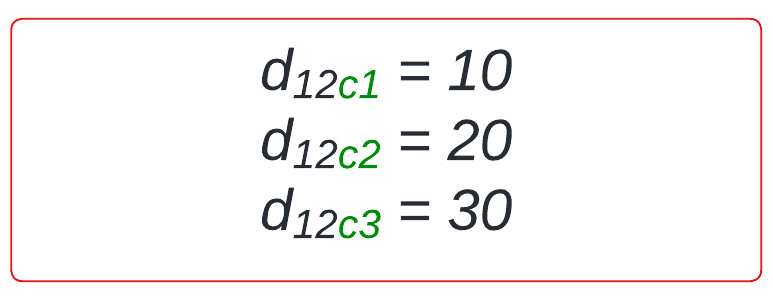
\includegraphics[width=\linewidth]{img/dem_indepen.png}
		\caption{Demanda Independente [$d$]}
		\label{fig:dem_indepen}
	\end{subfigure}\hspace{5mm}
	\begin{subfigure}[b]{0.40\linewidth}
		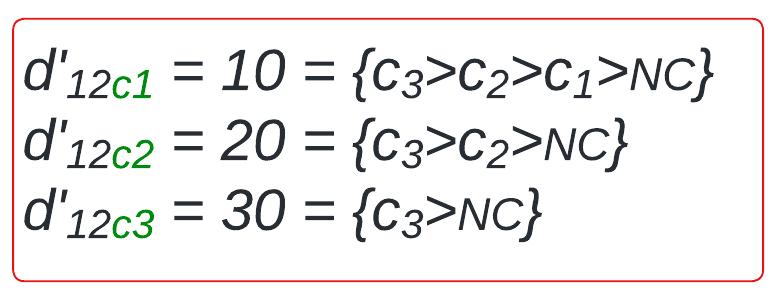
\includegraphics[width=\linewidth]{img/dem_compo.png}
		\caption{Demanda Comportamental [$d'$]}
		\label{fig:dem_comporta}
	\end{subfigure}
	\caption{Exemplo: Tipos de Demanda}
	\label{fig: tipos_demanda}
\end{figure}


Para interpretar a demanda independente, podemos dizer (segundo a Figura \ref{fig:dem_indepen}) que: existem 10 pessoas dispostas a comprar passagens \textbf{a um preço} de $c_1$, 20 pessoas a comprar \textbf{a um preço} de $c_2$ e 30 pessoas a comprar \textbf{a um preço} de $c_3$. No entanto, se as 10 pessoas dispostas a pagar $c_1$ encontrarem um melhor valor no momento da compra (por exemplo, $c_3$), essas pessoas prefeririam não comprar, situação que, na realidade, não faria sentido.

Por outro lado, temos a demanda comportamental, denotada como $d'$, que esta representada com uma lista de preferência, conforme visto na Figura \ref{fig:dem_comporta}. Esta lista significa que, por exemplo, 10 pessoas estão dispostas a comprar \textbf{até um preço} com valor $c_1$ (antes de preferir não comprar (NC)), 20 pessoas estão dispostas a comprar \textbf{até um preço} de $c_2$  (antes de preferir não comprar) e 30 pessoas estão dispostas a comprar \textbf{até um preço} de $c_3$  (antes de preferir não comprar).

O funcionamento seria o seguinte: imagine que as 10 pessoas dispostas a comprar até um valor de $c_1$ vão tentar comprar primeiro a um valor mais barato, neste caso $c_3$. Se $c_3$ não estiver disponível, elas procurariam assentos com valor $c_2$. Se $c_2$ também não estiver disponível, subiriam na lista e procurariam passagens com valor de $c_1$. Se estes não estiverem disponíveis, então não comprariam. Note que esse comportamento é o que comumente se usa na realidade.

Agora, analisa-se como o modelo interpretaria esse novo comportamento. Para isso, calcula-se a nova demanda potencial:

Para $c_1$, analisa-se a lista e verifica-se quem está disposto a pagar por esse valor.
\begin{figure}[H]
	\begin{center}
		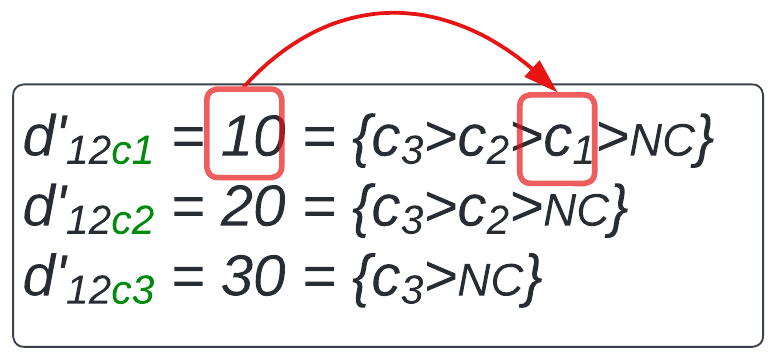
\includegraphics[scale=0.24]{img/dem_compo_c1.png}
		\caption{Exemplo: demanda comportamental para a classe $c_1$}
		% Fonte:~\cite{khaksar2013genetic}}
		\label{fig: exemplo_dem_c1}
	\end{center}
\end{figure}

Segundo a Figura \ref{fig: exemplo_dem_c1}, apenas 10 possíveis passageiros estão dispostos a pagar esse valor.

Agora, analisa-se quem está disposto a pagar um valor por um bilhete da classe $c_2$
\begin{figure}[H]
	\begin{center}
		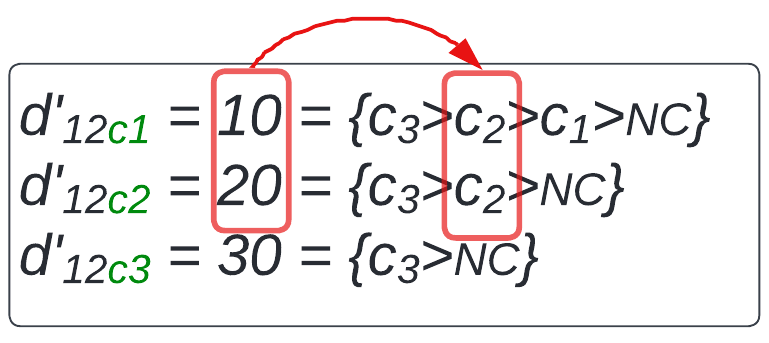
\includegraphics[scale=0.24]{img/dem_compo_c2.png}
		\caption{Exemplo: demanda comportamental para a classe $c_2$}
		% Fonte:~\cite{khaksar2013genetic}}
		\label{fig: exemplo_dem_c2}
	\end{center}
\end{figure}

Neste caso, 30 possíveis pessoas estariam dispostas a pagar esse valor. Observe que, de esta nova demanda, 10 pessoas correspondentes à demanda de $c_1$ também estariam dispostas a comprar pelo valor da classe $c_2$.

Por último, para a classe mais barata c3, veja a Figura \ref{fig: exemplo_dem_c3}.
\begin{figure}[H]
	\begin{center}
		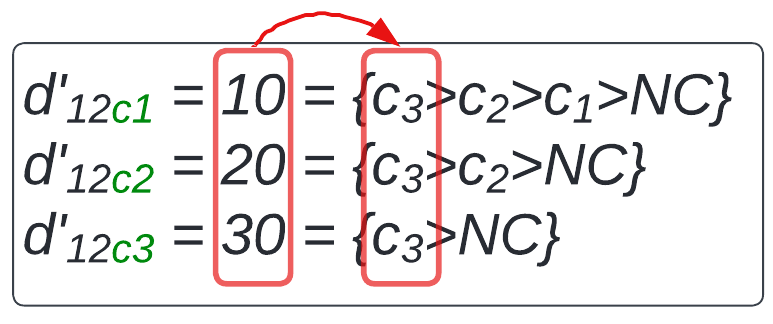
\includegraphics[scale=0.24]{img/dem_compo_c3.png}
		\caption{Exemplo: demanda comportamental para a classe $c_3$}
		% Fonte:~\cite{khaksar2013genetic}}
		\label{fig: exemplo_dem_c3}
	\end{center}
\end{figure}
Note que, neste caso, 60 pessoas estariam dispostas a pagar um bilhete da classe $c_3$, ou seja, toda a demanda do trecho $(E_1-E_2)$ compraria pelo valor mais barato se este estivesse disponível.

Assim, a demanda potencial comportamental para o modelo seria como se apresenta na Figura \ref{fig: exemplo_dem_poten}.
\begin{figure}[H]
	\begin{center}
		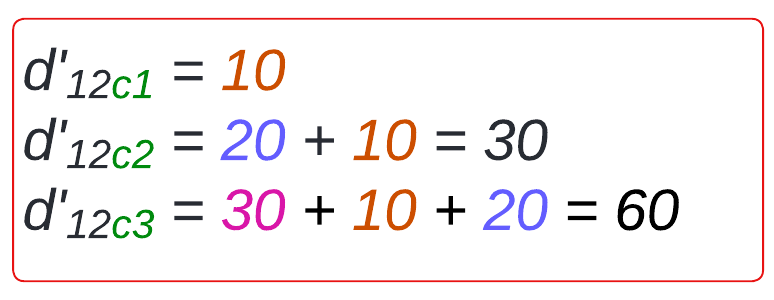
\includegraphics[scale=0.24]{img/dem_compo_poten.png}
		\caption{Exemplo: demanda comportamental total potencial}
		\label{fig: exemplo_dem_poten}
	\end{center}
\end{figure}
No entanto, é importante lembrar que a demanda potencial inicial era de 60 pessoas, mas até este ponto, a demanda poderia ser maior, pois a demanda de cada classe comercial agora é o acúmulo das demandas das classes mais caras. Essa situação precisa ser controlada para não criar uma demanda inexistente; para isso, serão consideradas as seguintes restrições, relacionando neste caso as variáveis de decisão de assentos reservados:
\begin{align}
	 & X_{12\textcolor[rgb]{0.0588, 0.5412, 0.4275}{c_1}} \leq d'_{12\textcolor[rgb]{0.0588, 0.5412, 0.4275}{c_1}} = 10                        \label{eq: dem_asiig_c1}                                                                                    \\
	 & X_{12\textcolor[rgb]{0.0588, 0.5412, 0.4275}{c_2}} \leq d'_{12\textcolor[rgb]{0.0588, 0.5412, 0.4275}{c_2}} = 30                        \label{eq: dem_asiig_c2}                                                                                    \\
	 & X_{12\textcolor[rgb]{0.0588, 0.5412, 0.4275}{c_3}} \leq d'_{12\textcolor[rgb]{0.0588, 0.5412, 0.4275}{c_3}} = 60                      \label{eq: dem_asiig_c3}                                                                                      \\
	 & X_{12\textcolor[rgb]{0.0588, 0.5412, 0.4275}{c_1}} + X_{12\textcolor[rgb]{0.0588, 0.5412, 0.4275}{c_2}} \leq d'_{12\textcolor[rgb]{0.0588, 0.5412, 0.4275}{c_2}}  = 30           \label{eq: dem_compo_c2}                                           \\
	 & X_{12\textcolor[rgb]{0.0588, 0.5412, 0.4275}{c_1}} + X_{12\textcolor[rgb]{0.0588, 0.5412, 0.4275}{c_2}} + X_{12\textcolor[rgb]{0.0588, 0.5412, 0.4275}{c_3}} \leq d'_{12\textcolor[rgb]{0.0588, 0.5412, 0.4275}{c_3}} = 60 \label{eq: dem_compo_c3}
\end{align}

Observe-se que as restrições de \ref{eq: dem_asiig_c1} até \ref{eq: dem_asiig_c3} são restrições conhecidas que limitam os valores que as passagens reservadas podem assumir, enquanto as restrições \ref{eq: dem_compo_c2} e \ref{eq: dem_compo_c3} são as que auxiliarão no controle para que não se ultrapasse a demanda potencial total inicial.

Por exemplo, se $X_{12\textcolor[rgb]{0.0588, 0.5412, 0.4275}{c_2}}$ assume o valor de 30 (restrição \ref{eq: dem_asiig_c2}), a restrição \ref{eq: dem_compo_c2} garante que $X_{12\textcolor[rgb]{0.0588, 0.5412, 0.4275}{c_1}}$ seja igual a 0, pois a demanda de 10 pessoas correspondente preferiu comprar ao preço da classe $c_2$. A mesma situação ocorreria se $X_{12\textcolor[rgb]{0.0588, 0.5412, 0.4275}{c_3}}$ assumisse o valor de 60 (restrição \ref{eq: dem_asiig_c3}), então a restrição \ref{eq: dem_compo_c3} garantiria que a demanda por $X_{12\textcolor[rgb]{0.0588, 0.5412, 0.4275}{c_1}}$ e $X_{12\textcolor[rgb]{0.0588, 0.5412, 0.4275}{c_2}}$ fosse igual a zero, já que esses clientes decidiram comprar pelo valor da classe $c_3$. Dessa forma, esse conjunto de restrições funcionaria para cada combinação possível das variáveis descritas.

Os modelos desta seção possuem grande semelhança com os modelos do abordaje com demanda independente, razão pela qual serão adotadas as mesmas definições de conjuntos, variáveis de decisão e parâmetros. Serão feitas as devidas anotações sempre que houver algum cambio ou ajuste necessário.

\subsection{Modelo básico comportamental} 
Este modelo compartilha as mesmas restrições do modelo básico com demanda independente, exceto pela restrição \eqref{eq: m1_assig_menor_dem}, que manterá a mesma estrutura, mas agora utilizando a demanda comportamental em vez da demanda independente.

Considere os seguintes parâmetros:
\begin{description}[style=unboxed, leftmargin=2.5cm, labelindent=1.5cm]
	\setlength{\itemsep}{-2.2em} % Ajusta el interlineado entre ítems
	\setlength{\parskip}{0em} % Espaciado entre párrafos
	\item[$d'_{ijvkt}:$] Demanda comportamental no trecho $(i,j)$, tipo de assento $v$ e classe de controle $k$, onde $(i,j) \in OD,v \in V, k \in K_v, t \in T$.\\
	\item[$M:$] É um número suficientemente grande.\\
	\item[$\sigma_{ijvkt}:$] é a probabilidade (baseada na simulação de Monte Carlo) de que um passageiro disposto a pagar o valor do bilhete da classe $k$ e tipo de assento $v$ chegue no período $t$ do trecho $(i,j)$. Onde $(i,j) \in OD,v \in V, k \in K_v, t \in T$.
\end{description}

Considere as seguintes variáveis de decisão:
\begin{description}[style=unboxed, leftmargin=2.5cm, labelindent=1.5cm]
	\setlength{\itemsep}{-2.2em} % Ajusta el interlineado entre ítems
	\setlength{\parskip}{0em} % Espaciado entre párrafos
	    \item[$\delta_{ijvkt}:$] Delta é uma variável binária que assume o valor de 1 quando o preço da classe mais cara é maior do que a soma dos preços das classes mais baratas, e o valor de 0 em caso contrário., onde $(i,j) \in OD, v \in V, k=min\{K_v\}, t \in T$.
\end{description}


\textbf{Modelo}
\begin{equation}
	Max \quad Z = \sum_{(i,j)\in OD} \sum_{v\in V} \sum_{k\in K_v} \sum_{t\in T} \sigma_{ijvkt} P_{ijvk} X_{ijvkt}           \label{eq: fo_beha}
\end{equation}
Agora, a função objetivo \eqref{eq: fo_beha} leva em consideração a probabilidade de chegada de um possível passageiro para cada classe de controle, em cada período, tipo de assento e trecho específico.
\begin{equation}
	X_{ijvkt} \leq d'_{ijvkt},  \quad \forall (i,j) \in OD / i < j  ,v \in V, k \in K_v, t\in T  \label{eq: rel_x_dem_beha}
\end{equation}
Note-se que a restrição \eqref{eq: rel_x_dem_beha} está limitando a quantidade de assentos reservados, de forma que estes não ultrapassem o valor da demanda comportamental.
\begin{equation}
	\sum_{k' \in K_v / k' \leq k}X_{i,j,v,k',t} \leq d'_{ijvkt} \quad \forall (i,j) \in OD, v \in V, k \in K_v / k > 1, t\in T     \label{eq: dem_compor_acumulacao_class}
\end{equation}
A restrição \eqref{eq: dem_compor_acumulacao_class} é a generalização da situação explicada pelas restrições \eqref{eq: dem_compo_c2}  e \eqref{eq: dem_compo_c3}.

Apenas adicionando as duas restrições, \eqref{eq: rel_x_dem_beha} e \eqref{eq: dem_compor_acumulacao_class}, e eliminando a restrição \eqref{eq: m1_assig_menor_dem} do modelo básico independente, obteríamos, em teoria, um modelo com demanda comportamental. No entanto, essa afirmação não é completamente verdadeira. Embora as novas restrições limitem a demanda do modelo de maneira que seja possível utilizar as listas de preferência, o modelo ainda se comportará como um modelo independente.

Isso ocorre porque a demanda independente é um caso particular de todas as combinações possíveis que podem ser geradas ao usar as listas de preferência. De fato, a demanda independente é o caso que geraria o maior lucro possível entre todas essas combinações. Vale lembrar que as listas de preferência oferecem a flexibilidade de permitir que um cliente disposto a pagar mais caro adquira um produto a um preço mais barato, caso essa possibilidade exista.

Portanto, é necessário, de alguma forma, informar ao modelo que ele deve considerar outras possibilidades "mais realistas" \, durante a resolução do problema.
\begin{gather}
	\alpha_{ijvkt} +  \sum_{k' \in K_v / k'>k}  \alpha_{i,j,v,k',t}  \leq 1+M(1-\delta_{ijvkt}), \quad   k = min\{K_v\}, \forall(i,j) \in OD, v \in V, t \in T  \label{eq: ajuste1} \\
	\begin{split}
		\sigma_{ijvkt} P_{ijvk}X_{ijvkt} + M(1-\delta_{ijvkt})   \geq \sum_{k' \in K_v / k'>k} \sigma_{ijvkt} P_{i,j,v,k'}X_{i,j,v,k',t}, \\  k = min\{K_v\}, \forall(i,j) \in OD, v \in V, t \in T  \label{eq: ajuste2}
	\end{split} \\
	\alpha_{ijvkt} \leq \delta_{ijvkt}, \quad   k = min\{K_v\}, \forall(i,j) \in OD, v \in V, t \in T   \label{eq: ajuste3}
\end{gather}
Dessa forma, as restrições  \eqref{eq: ajuste1},  \eqref{eq: ajuste2} e  \eqref{eq: ajuste3} atuam de maneira integrada para realizar o ajuste necessário. Esse ajuste consiste em identificar a classe mais cara e verificar se seu preço é superior à soma dos preços das classes mais baratas. Se a condição for verdadeira, as classes mais baratas serão desabilitadas, e apenas a classe mais cara será mantida. Caso contrário, o modelo permanecerá livre para selecionar a opção mais vantajosa, de acordo com as condições estabelecidas.

Assim, o \textbf{modelo básico} seria o seguinte:
\allowdisplaybreaks
\begin{align}
	& Max \quad Z = \sum_{(i,j)\in OD} \sum_{v\in V} \sum_{k\in K_v} \sum_{t\in T} P_{ijvk} X_{ijvkt}     \tag{\ref{eq: m1_fo}}   \\
	& \text{s.a.}  \notag \\
	& A_{iv} = A_{i-1,v} - \sum_{(i,j) \in OD/j \geq i} \sum_{k\in K_v}\sum_{t\in T}X_{i-1,j,v,k,t} + \sum_{(i,j) \in OD/j<i} \sum_{k\in K_v}\sum_{t\in T}X_{jivkt}, \quad \forall i \in O, v \in V   \tag{\ref{eq: m1_disponi}} \\
	& Y_{ijvk} \geq  \sum_{t \in T} X_{ijvkt},  \quad k = max\{K_v\}, \forall(i,j) \in OD ,v \in V     \tag{\ref{eq: m1_autho_mayor_assig_1er_class}} \\
	& Y_{ijvk} \geq  \sum_{t \in T} X_{ijvkt} + Y_{i,j,v,k + 1} , \quad \forall(i,j) \in OD, v \in V, k \in K_v / k < \lVert K_v \rVert   \tag{\ref{eq: m1_autho_mayor_assig_mas_autho}} \\
	& \sum_{(i,j) \in OD} Y_{ijvk} \leq A_{iv}, \quad  k = min\{K_v\}, \forall i \in O / (i,j) \in OD,   \forall v \in V       \tag{\ref{eq: m1_cap_autho_1er_class}} \\
	% & X_{ijvkt} \leq d_{ijvkt},  \quad \forall (i,j) \in OD / i < j  ,v \in V, k \in K_v, t\in T   \tag{\ref{eq: m1_assig_menor_dem}} \\
	& A_{0,v} = Q_v \quad \forall v \in V  \tag{\ref{eq: m1_ini_disponi}} \\ 
	& X_{0,j,v,k,t} = 0 \quad \forall j \in D,\, v \in V,\, k \in K_v,\, t \in T  \tag{\ref{eq: m1_ini_assig}} \\ 
	& X_{ijvkt} \in \mathbb{Z}^+ \quad \forall(i,j) \in OD,\, v \in V,\, k \in K_v,\, t \in T  \tag{\ref{eq: m1_dom_assig}} \\ 
	& Y_{ijvk} \in \mathbb{Z}^+ \quad \forall(i,j) \in OD,\, v \in V,\, k \in K_v  \tag{\ref{eq: m1_dom_autho}} \\ 
	& A_{iv} \in \mathbb{Z}^+ \quad \forall i \in O,\, v \in V  \tag{\ref{eq: m1_dom_disponi}} \\
	& \textit{\underline{Restrições demanda comportamental}}         \notag   \\
	& X_{ijvkt} \leq d'_{ijvkt},  \quad \forall (i,j) \in OD / i < j  ,v \in V, k \in K_v, t\in T   \tag{\ref{eq: rel_x_dem_beha}} \\
	& \sum_{k' \in K_v / k' \leq k}X_{i,j,v,k',t} \leq d'_{ijvkt} \quad \forall (i,j) \in OD, v \in V, k \in K_v / k > 1, t\in T     \tag{\ref{eq: dem_compor_acumulacao_class}} \\
	& \textit{\underline{Restrições ajuste da demanda}}         \notag   \\
	& \alpha_{ijvkt} +  \sum_{k' \in K_v / k'>k}  \alpha_{i,j,v,k',t}  \leq 1+M(1-\delta_{ijvkt}), \quad   k = min\{K_v\}, \forall(i,j) \in OD, v \in V, t \in T  \tag{\ref{eq: ajuste1}} \\
	\begin{split}
		& \sigma_{ijvk}P_{ijvk}X_{ijvkt} + M(1-\delta_{ijvkt})   \geq \sum_{k' \in K_v / k'>k} \sigma_{ijvk} P_{i,j,v,k'}X_{i,j,v,k',t}, \\  
		& k = min\{K_v\}, \forall(i,j) \in OD, v \in V, t \in T  
	\end{split} \tag{\ref{eq: ajuste2}} \\
	& \alpha_{ijvkt} \leq \delta_{ijvkt}, \quad   k = min\{K_v\}, \forall(i,j) \in OD, v \in V, t \in T   \tag{\ref{eq: ajuste3}}
\end{align}

\subsection{Modelo fulfillments over periods comportamental}
Todos os parâmetros, conjuntos, variáveis de decisão e restrições foram detalhadamente explicados nas seções anteriores. Por tanto, nesta seção, somente são adicionadas as restrições de fulfillment, criadas no modelo independente, ao modelo comportamental básico apresentado na seção anterior.
\allowdisplaybreaks
\begin{align}
	& Max \quad Z = \sum_{(i,j)\in OD} \sum_{v\in V} \sum_{k\in K_v} \sum_{t\in T} P_{ijvk} X_{ijvkt}     \tag{\ref{eq: m1_fo}}   \\
	& \text{s.a.}  \notag \\
	& A_{iv} = A_{i-1,v} - \sum_{(i,j) \in OD/j \geq i} \sum_{k\in K_v}\sum_{t\in T}X_{i-1,j,v,k,t} + \sum_{(i,j) \in OD/j<i} \sum_{k\in K_v}\sum_{t\in T}X_{jivkt}, \quad \forall i \in O, v \in V   \tag{\ref{eq: m1_disponi}} \\
	& Y_{ijvk} \geq  \sum_{t \in T} X_{ijvkt},  \quad k = max\{K_v\}, \forall(i,j) \in OD ,v \in V     \tag{\ref{eq: m1_autho_mayor_assig_1er_class}} \\
	& Y_{ijvk} \geq  \sum_{t \in T} X_{ijvkt} + Y_{i,j,v,k + 1} , \quad \forall(i,j) \in OD, v \in V, k \in K_v / k < \lVert K_v \rVert   \tag{\ref{eq: m1_autho_mayor_assig_mas_autho}} \\
	& \sum_{(i,j) \in OD} Y_{ijvk} \leq A_{iv}, \quad  k = min\{K_v\}, \forall i \in O / (i,j) \in OD,   \forall v \in V       \tag{\ref{eq: m1_cap_autho_1er_class}} \\
	% & X_{ijvkt} \leq d_{ijvkt},  \quad \forall (i,j) \in OD / i < j  ,v \in V, k \in K_v, t\in T   \tag{\ref{eq: m1_assig_menor_dem}} \\
	& A_{0,v} = Q_v \quad \forall v \in V  \tag{\ref{eq: m1_ini_disponi}} \\ 
	& X_{0,j,v,k,t} = 0 \quad \forall j \in D,\, v \in V,\, k \in K_v,\, t \in T  \tag{\ref{eq: m1_ini_assig}} \\ 
	& X_{ijvkt} \in \mathbb{Z}^+ \quad \forall(i,j) \in OD,\, v \in V,\, k \in K_v,\, t \in T  \tag{\ref{eq: m1_dom_assig}} \\ 
	& Y_{ijvk} \in \mathbb{Z}^+ \quad \forall(i,j) \in OD,\, v \in V,\, k \in K_v  \tag{\ref{eq: m1_dom_autho}} \\ 
	& A_{iv} \in \mathbb{Z}^+ \quad \forall i \in O,\, v \in V  \tag{\ref{eq: m1_dom_disponi}} \\
	& \textit{\underline{Restrições demanda comportamental}}         \notag   \\
	& X_{ijvkt} \leq d'_{ijvkt},  \quad \forall (i,j) \in OD / i < j  ,v \in V, k \in K_v, t\in T   \tag{\ref{eq: rel_x_dem_beha}} \\
	& \sum_{k' \in K_v / k' \leq k}X_{i,j,v,k',t} \leq d'_{ijvkt} \quad \forall (i,j) \in OD, v \in V, k \in K_v / k > 1, t\in T     \tag{\ref{eq: dem_compor_acumulacao_class}} \\
	& \textit{\underline{Restrições ajuste da demanda}}         \notag   \\
	& \alpha_{ijvkt} +  \sum_{k' \in K_v / k'>k}  \alpha_{i,j,v,k',t}  \leq 1+M(1-\delta_{ijvkt}), \quad   k = min\{K_v\}, \forall(i,j) \in OD, v \in V, t \in T  \tag{\ref{eq: ajuste1}} \\
	\begin{split}
		& \sigma_{ijvk}P_{ijvk}X_{ijvkt} + M(1-\delta_{ijvkt})   \geq \sum_{k' \in K_v / k'>k} \sigma_{ijvk} P_{i,j,v,k'}X_{i,j,v,k',t}, \\  
		& k = min\{K_v\}, \forall(i,j) \in OD, v \in V, t \in T  
	\end{split} \tag{\ref{eq: ajuste2}} \\
	& \alpha_{ijvkt} \leq \delta_{ijvkt}, \quad   k = min\{K_v\}, \forall(i,j) \in OD, v \in V, t \in T   \tag{\ref{eq: ajuste3}} \\
	& \textit{\underline{Restrições fulfillments over periods}}         \notag   \\
	& \alpha_{ijvkt} \leq X_{ijvkt} \leq \alpha_{ijvkt}d_{ijvkt}, \quad   \forall(i,j) \in OD, v \in V, k \in K_v, t \in T   \tag{\ref{eq: m1_binaria_alpha}} \\
	& \beta_{ijvkt} = \alpha_{ijvkt} - \alpha_{i,j,v,k+1,t}, \quad \forall (i,j) \in OD, v \in V, k \in K /k < max\{K_v\}, t\in T    \tag{\ref{eq: m1_binaria_Beta}}   \\
	& \beta_{ijvkt} = \alpha_{ijvkt}, \quad   \forall(i,j) \in OD, v \in V, k = max\{K_v\}, t \in T    \tag{\ref{eq: m1_binaria_Beta_last}}   \\
	& \alpha_{ijvkt} \leq \alpha_{i,j,v,k,t+1}, \quad   \forall(i,j) \in OD, v \in V, k \in K_v, t \in T/ t \neq max\{T\}     \tag{\ref{eq: m1_assig_last_periodo}}   \\
	& \sum_{k \in K_v}\beta_{ijvkt}P_{ijvk} \geq \sum_{k \in K_v}\beta_{i,j,v,k,t+1}P_{ijvk},  \quad   \forall(i,j) \in OD, v \in V, t \in T/ t \neq max\{T\}   \tag{\ref{eq: m1_fulfill_periodo}}
\end{align}


\subsection{Modelo skip lagging comportamental}
De maneira análoga ao modelo fulfillment over periods, nesta seção, são incorporadas as restrições de skip lagging, do modelo independente, ao modelo comportamental básico.
\allowdisplaybreaks
\begin{align}
	& Max \quad Z = \sum_{(i,j)\in OD} \sum_{v\in V} \sum_{k\in K_v} \sum_{t\in T} P_{ijvk} X_{ijvkt}     \tag{\ref{eq: m1_fo}}   \\
	& \text{s.a.}  \notag \\
	& A_{iv} = A_{i-1,v} - \sum_{(i,j) \in OD/j \geq i} \sum_{k\in K_v}\sum_{t\in T}X_{i-1,j,v,k,t} + \sum_{(i,j) \in OD/j<i} \sum_{k\in K_v}\sum_{t\in T}X_{jivkt}, \quad \forall i \in O, v \in V   \tag{\ref{eq: m1_disponi}} \\
	& Y_{ijvk} \geq  \sum_{t \in T} X_{ijvkt},  \quad k = max\{K_v\}, \forall(i,j) \in OD ,v \in V     \tag{\ref{eq: m1_autho_mayor_assig_1er_class}} \\
	& Y_{ijvk} \geq  \sum_{t \in T} X_{ijvkt} + Y_{i,j,v,k + 1} , \quad \forall(i,j) \in OD, v \in V, k \in K_v / k < \lVert K_v \rVert   \tag{\ref{eq: m1_autho_mayor_assig_mas_autho}} \\
	& \sum_{(i,j) \in OD} Y_{ijvk} \leq A_{iv}, \quad  k = min\{K_v\}, \forall i \in O / (i,j) \in OD,   \forall v \in V       \tag{\ref{eq: m1_cap_autho_1er_class}} \\
	% & X_{ijvkt} \leq d_{ijvkt},  \quad \forall (i,j) \in OD / i < j  ,v \in V, k \in K_v, t\in T   \tag{\ref{eq: m1_assig_menor_dem}} \\
	& A_{0,v} = Q_v \quad \forall v \in V  \tag{\ref{eq: m1_ini_disponi}} \\ 
	& X_{0,j,v,k,t} = 0 \quad \forall j \in D,\, v \in V,\, k \in K_v,\, t \in T  \tag{\ref{eq: m1_ini_assig}} \\ 
	& X_{ijvkt} \in \mathbb{Z}^+ \quad \forall(i,j) \in OD,\, v \in V,\, k \in K_v,\, t \in T  \tag{\ref{eq: m1_dom_assig}} \\ 
	& Y_{ijvk} \in \mathbb{Z}^+ \quad \forall(i,j) \in OD,\, v \in V,\, k \in K_v  \tag{\ref{eq: m1_dom_autho}} \\ 
	& A_{iv} \in \mathbb{Z}^+ \quad \forall i \in O,\, v \in V  \tag{\ref{eq: m1_dom_disponi}} \\
	& \textit{\underline{Restrições demanda comportamental}}         \notag   \\
	& X_{ijvkt} \leq d'_{ijvkt},  \quad \forall (i,j) \in OD / i < j  ,v \in V, k \in K_v, t\in T   \tag{\ref{eq: rel_x_dem_beha}} \\
	& \sum_{k' \in K_v / k' \leq k}X_{i,j,v,k',t} \leq d'_{ijvkt} \quad \forall (i,j) \in OD, v \in V, k \in K_v / k > 1, t\in T     \tag{\ref{eq: dem_compor_acumulacao_class}} \\
	& \textit{\underline{Restrições ajuste da demanda}}         \notag   \\
	& \alpha_{ijvkt} +  \sum_{k' \in K_v / k'>k}  \alpha_{i,j,v,k',t}  \leq 1+M(1-\delta_{ijvkt}), \quad   k = min\{K_v\}, \forall(i,j) \in OD, v \in V, t \in T  \tag{\ref{eq: ajuste1}} \\
	\begin{split}
		& \sigma_{ijvk}P_{ijvk}X_{ijvkt} + M(1-\delta_{ijvkt})   \geq \sum_{k' \in K_v / k'>k} \sigma_{ijvk} P_{i,j,v,k'}X_{i,j,v,k',t}, \\  
		& k = min\{K_v\}, \forall(i,j) \in OD, v \in V, t \in T  
	\end{split} \tag{\ref{eq: ajuste2}} \\
	& \alpha_{ijvkt} \leq \delta_{ijvkt}, \quad   k = min\{K_v\}, \forall(i,j) \in OD, v \in V, t \in T   \tag{\ref{eq: ajuste3}} \\
	& \textit{\underline{Restrições skip lagging}}         \notag   \\
	& \alpha_{ijvkt} \leq X_{ijvkt} \leq \alpha_{ijvkt}d_{ijvkt}, \quad   \forall(i,j) \in OD, v \in V, k \in K_v, t \in T   \tag{\ref{eq: m1_binaria_alpha}} \\
	& \beta_{ijvkt} = \alpha_{ijvkt} - \alpha_{i,j,v,k+1,t}, \quad \forall (i,j) \in OD, v \in V, k \in K /k < max\{K_v\}, t\in T    \tag{\ref{eq: m1_binaria_Beta}}   \\
	& \beta_{ijvkt} = \alpha_{ijvkt}, \quad   \forall(i,j) \in OD, v \in V, k = max\{K_v\}, t \in T    \tag{\ref{eq: m1_binaria_Beta_last}}   \\
	& \sum_{k \in K_v}\beta_{ijvkt}P_{ijvk} \leq \sum_{k \in K_v}\beta_{i,j',v,k,t}P_{ijvk}, \quad \forall i \in O, j \in D, j' \in D / j' > j, v \in V, t \in T    \tag{\ref{eq: m1_preco_estacao_inicio}}   \\
	\begin{split}
		& \sum_{k \in K_v}\beta_{odvkt}P_{odvk} \leq \sum_{(i,j) \in S}\sum_{k \in K_v}\beta_{ijvkt}P_{ijvk}, \quad    \forall (o,d) \in NAD, \\
		& v \in V, t \in T , \quad  \forall S \in CR_{o,d} / S \subset CR_{o,d}     \\
	\end{split}   \tag{\ref{eq: m1_preco_combinacao_rotas_contidas}}
\end{align}


\subsection{Modelo completo comportamental}
Nesta seção, integramos o modelo comportamental base com os conjuntos de restrições de fulfillment over periods e skip lagging, incorporando todos os elementos de forma simultânea.
\allowdisplaybreaks
\begin{align}
	& Max \quad Z = \sum_{(i,j)\in OD} \sum_{v\in V} \sum_{k\in K_v} \sum_{t\in T} P_{ijvk} X_{ijvkt}     \tag{\ref{eq: m1_fo}}   \\
	& \text{s.a.}  \notag \\
	& A_{iv} = A_{i-1,v} - \sum_{(i,j) \in OD/j \geq i} \sum_{k\in K_v}\sum_{t\in T}X_{i-1,j,v,k,t} + \sum_{(i,j) \in OD/j<i} \sum_{k\in K_v}\sum_{t\in T}X_{jivkt}, \quad \forall i \in O, v \in V   \tag{\ref{eq: m1_disponi}} \\
	& Y_{ijvk} \geq  \sum_{t \in T} X_{ijvkt},  \quad k = max\{K_v\}, \forall(i,j) \in OD ,v \in V     \tag{\ref{eq: m1_autho_mayor_assig_1er_class}} \\
	& Y_{ijvk} \geq  \sum_{t \in T} X_{ijvkt} + Y_{i,j,v,k + 1} , \quad \forall(i,j) \in OD, v \in V, k \in K_v / k < \lVert K_v \rVert   \tag{\ref{eq: m1_autho_mayor_assig_mas_autho}} \\
	& \sum_{(i,j) \in OD} Y_{ijvk} \leq A_{iv}, \quad  k = min\{K_v\}, \forall i \in O / (i,j) \in OD,   \forall v \in V       \tag{\ref{eq: m1_cap_autho_1er_class}} \\
	% & X_{ijvkt} \leq d_{ijvkt},  \quad \forall (i,j) \in OD / i < j  ,v \in V, k \in K_v, t\in T   \tag{\ref{eq: m1_assig_menor_dem}} \\
	& A_{0,v} = Q_v \quad \forall v \in V  \tag{\ref{eq: m1_ini_disponi}} \\ 
	& X_{0,j,v,k,t} = 0 \quad \forall j \in D,\, v \in V,\, k \in K_v,\, t \in T  \tag{\ref{eq: m1_ini_assig}} \\ 
	& X_{ijvkt} \in \mathbb{Z}^+ \quad \forall(i,j) \in OD,\, v \in V,\, k \in K_v,\, t \in T  \tag{\ref{eq: m1_dom_assig}} \\ 
	& Y_{ijvk} \in \mathbb{Z}^+ \quad \forall(i,j) \in OD,\, v \in V,\, k \in K_v  \tag{\ref{eq: m1_dom_autho}} \\ 
	& A_{iv} \in \mathbb{Z}^+ \quad \forall i \in O,\, v \in V  \tag{\ref{eq: m1_dom_disponi}} \\
	& \textit{\underline{Restrições demanda comportamental}}         \notag   \\
	& X_{ijvkt} \leq d'_{ijvkt},  \quad \forall (i,j) \in OD / i < j  ,v \in V, k \in K_v, t\in T   \tag{\ref{eq: rel_x_dem_beha}} \\
	& \sum_{k' \in K_v / k' \leq k}X_{i,j,v,k',t} \leq d'_{ijvkt} \quad \forall (i,j) \in OD, v \in V, k \in K_v / k > 1, t\in T     \tag{\ref{eq: dem_compor_acumulacao_class}} \\
	& \textit{\underline{Restrições ajuste da demanda}}         \notag   \\
	& \alpha_{ijvkt} +  \sum_{k' \in K_v / k'>k}  \alpha_{i,j,v,k',t}  \leq 1+M(1-\delta_{ijvkt}), \quad   k = min\{K_v\}, \forall(i,j) \in OD, v \in V, t \in T  \tag{\ref{eq: ajuste1}} \\
	\begin{split}
		& \sigma_{ijvk}P_{ijvk}X_{ijvkt} + M(1-\delta_{ijvkt})   \geq \sum_{k' \in K_v / k'>k} \sigma_{ijvk} P_{i,j,v,k'}X_{i,j,v,k',t}, \\  
		& k = min\{K_v\}, \forall(i,j) \in OD, v \in V, t \in T  
	\end{split} \tag{\ref{eq: ajuste2}} \\
	& \alpha_{ijvkt} \leq \delta_{ijvkt}, \quad   k = min\{K_v\}, \forall(i,j) \in OD, v \in V, t \in T   \tag{\ref{eq: ajuste3}} \\
	& \textit{\underline{Restrições fulfillments over periods}}         \notag   \\
	& \alpha_{ijvkt} \leq X_{ijvkt} \leq \alpha_{ijvkt}d_{ijvkt}, \quad   \forall(i,j) \in OD, v \in V, k \in K_v, t \in T   \tag{\ref{eq: m1_binaria_alpha}} \\
	& \beta_{ijvkt} = \alpha_{ijvkt} - \alpha_{i,j,v,k+1,t}, \quad \forall (i,j) \in OD, v \in V, k \in K /k < max\{K_v\}, t\in T    \tag{\ref{eq: m1_binaria_Beta}}   \\
	& \beta_{ijvkt} = \alpha_{ijvkt}, \quad   \forall(i,j) \in OD, v \in V, k = max\{K_v\}, t \in T    \tag{\ref{eq: m1_binaria_Beta_last}}   \\
	& \alpha_{ijvkt} \leq \alpha_{i,j,v,k,t+1}, \quad   \forall(i,j) \in OD, v \in V, k \in K_v, t \in T/ t \neq max\{T\}     \tag{\ref{eq: m1_assig_last_periodo}}   \\
	& \sum_{k \in K_v}\beta_{ijvkt}P_{ijvk} \geq \sum_{k \in K_v}\beta_{i,j,v,k,t+1}P_{ijvk},  \quad   \forall(i,j) \in OD, v \in V, t \in T/ t \neq max\{T\}   \tag{\ref{eq: m1_fulfill_periodo}} \\
	& \textit{\underline{Restrições skip lagging}}         \notag   \\
	& \sum_{k \in K_v}\beta_{ijvkt}P_{ijvk} \leq \sum_{k \in K_v}\beta_{i,j',v,k,t}P_{ijvk}, \quad \forall i \in O, j \in D, j' \in D / j' > j, v \in V, t \in T    \tag{\ref{eq: m1_preco_estacao_inicio}}   \\
	\begin{split}
		& \sum_{k \in K_v}\beta_{odvkt}P_{odvk} \leq \sum_{(i,j) \in S}\sum_{k \in K_v}\beta_{ijvkt}P_{ijvk}, \quad    \forall (o,d) \in NAD, \\
		& v \in V, t \in T , \quad  \forall S \in CR_{o,d} / S \subset CR_{o,d}     \\
	\end{split}   \tag{\ref{eq: m1_preco_combinacao_rotas_contidas}}
\end{align}
